\documentclass[11pt]{article}
\usepackage{amsmath,amssymb,amsthm}
\usepackage{graphicx}
\graphicspath{{./}}
\usepackage[margin=1in]{geometry}
\usepackage{fancyhdr}
\usepackage{listings}
\lstset{language=R}
\setlength{\parindent}{0pt}
\setlength{\parskip}{5pt plus 1pt}
\setlength{\headheight}{13.6pt}
\newcommand\question[2]{\vspace{.25in}\hrule\textbf{#1: #2}\vspace{.5em}\vspace{.10in}}
\renewcommand\part[1]{\vspace{.10in}\textbf{(#1)}}
\newcommand\algorithm{\vspace{.10in}\textbf{Algorithm: }}
\newcommand\correctness{\vspace{.10in}\textbf{Correctness: }}
\newcommand\runtime{\vspace{.10in}\textbf{Running time: }}
\pagestyle{fancyplain}
\lhead{\textbf{\NAME }}
\chead{\textbf{HW\HWNUM}}
\rhead{02-713, \today}
\begin{document}\raggedright
%Section A==============Change the values below to match your information==================
\newcommand\NAME{Jonathan Lopez}  % your name
\newcommand\HWNUM{4}              % the homework number
%Section B==============Put your answers to the questions below here=======================



\question{3.10.4}
{A random sample of size 5 is drawn from the pdf
    $f_{Y}(y)=2y, 0 \leq y \leq 1$
. Calculate
$P(Y_{1}' < 0.6 < Y_{5}')$
. \emph{Hint.} Consider the complement.}
\\
$
F_{Y}(y) 
=
\int_{0}^{y} 2y\ dy
=
y^{2} \big |_{0}^{y}
=
y^{2}
$
\\
$
f_{Y_{1}'}(y)
=
5[1-y^{2}]^{4} \ 2y
=
10y^{9} - 40y^{7} + 60y^{5} - 40y^{3} + 10y
$
\\
$
F_{Y_{1}'}
=
y^{10} - 5y^{8} + 10y^{6} - 10y^{4} + 5y^{2}
$
\\
$
f_{Y_{5}'}(y)
=
5[y^{2}]^{4} \ 2y
=
10y^9
$
\\
$
F_{Y_{5}'}
=
y^{10}
$
\\
$
P(Y_{1}' < 0.6 < Y_{5}')
=
[1-P(Y_{1}' \geq 0.6)] * [1-P(Y_{5}' \leq 0.6)]
$
\\
$
P(Y_{1}' \geq 0.6) 
=
\int_{0.6}^{1} y^{10} - 5y^{8} + 10y^{6} - 10y^{4} + 5y^{2} \ dt
=
\frac{y^{11}}{11} - 
\frac{5y^{9}}{9} + 
\frac{10y^{7}}{7} - 
\frac{10y^{5}}{5} + 
\frac{5y^{3}}{3}
\big |_{0.6}^{1}
=
0.3913
$
\\
$
P(Y_{5}' \leq 0.6)
=
\int_{0}^{0.6} y^{10} \ dt
=
\frac{y^{11}}{11} \big |_{0}^{0.6}
=
0.0906
$
\\
$
P(Y_{1}' < 0.6 < Y_{5}')
=
[1- 0.3913] * [1-0.0906]
=
0.5535
$
\\
Simulation:
\\
\begin{lstlisting}
prob_3_10_4 <- function(trials) {
    results = integer(trials)
    for(i in 1:trials){
        u = runif(5)
        y_inv = sort(sqrt(u)) # Inverse of y^2
        if(y_inv[1]<0.6 && y_inv[5]>0.6){
            results[i]=1
        }
    }
    mean(results)
}
\end{lstlisting}


\question{3.10.6}
{Let $Y_{1}$,$Y_{2}$,...,$Y_{n}$, be a random sample from the exponential pdf
$f_{Y}(y) = e^{-y},y \geq 0$.What is the smallest $n$ for which
$P(Y_{min} < 0.2) > 0.9$?
}
\\
$
F_{Y}(y) 
=
\int_{0}^{y} e^{-y} \ dt
=
-e^{-y} \big |_{0}^{y}
=
1 -e^{-y}
$
\\
$
f_{Y_{1}'}(y)
=
n[1-(1-e^{-y}]^{n-1} \ e^{-y}
=
ne^{y(2-n)}
$
\\
$
F_{Y_{1}'}(y)
=
\int_{0}^{0.2} ne^{y(2-n)} dy
=
\frac{ne^{y(2-n)}}{2-n} \big |_{0}^{0.2}
=
\frac{ne^{0.2(n-2)} - n}{2-n} 
$
\\
$
n=7,
F_{Y_{1}'}(y)
=
0.885
$
\\
$
n=8,
F_{Y_{1}'}(y)
=
0.932
$
\\
\emph{n=8}
\\
Simulation:
\\
\begin{lstlisting}
 prob_3_10_6 <- function(trials) {
    for(n in 1:20) {
        results = integer(trials)
        for (i in 1:trials) {
            u = runif(n)
            y_inv = sort(-log(u)) # Inverse of e^-y
            if (y_inv[1] < 0.2) {
                results[i] = 1
            }
            if (mean(results) > 0.9) {
                return(n)
            }
        }
    }
}
\end{lstlisting}


\question{3.10.8}
{A random sample of size $n = 5$ is drawn from the pdf
$f_{Y}(y) = 2y, 0 \leq y \leq 1$.
On the same set of axes, graph the pdf for
$Y_{2}$, $Y_{1}'$, and $Y_{5}'$.}
\\
$
Y_{2} = y^{2}
\ \ \ \ \ \ \ \ \ \ \ 
Y_{1}' = y^{10} - 5y^{8} + 10y^{6} - 10y^{4} + 5y^{2}
\ \ \ \ \ \ \ \ \ \ \ 
Y_{5}' = y^{10}
$
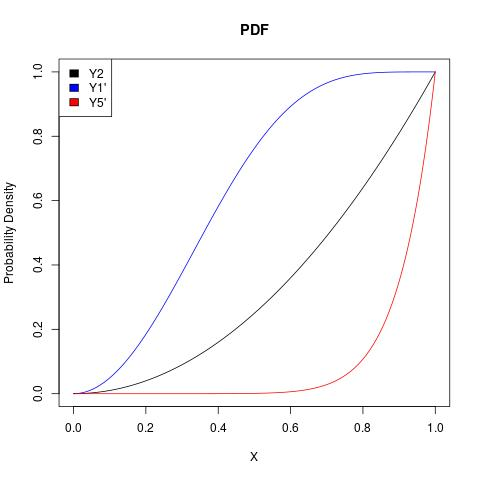
\includegraphics[scale=0.5]{rplot}


\question{3.10.10}
{Suppose that n observations are chosen at random from a continuous pdf
$f_{Y}(y)$
. What is the probability that the last observation recorded will be the smallest
number in the entire sample?}
\\
Sample Space: $n!$ ways
\\
nth observation is smallest: $(n-1)!$ ways
\\
P(Last Observation is Smallest Observation) = $\frac{(n-1)!}{n!} = \frac{1}{n}$


% \question{3.10.12}
% {Consider a system containing $n$ components, where the lifetimes of the 
% components are inependent random variables and each has pdf
% $f_{Y}(y) = \lambda e^{- \lambda y}, y > 0$
% . Show that the average time elapsing before the first component failure occurs
% is $1/n \lambda $.}


\question{3.12.4}
{Find the moment-generating function for the discrete random variable $X$
whose probability function is given by
$p_{x}(k) = (\frac{3}{4})^{k}(\frac{1}{4}), k = 0,1,2...$}
\\
$
M_{X}(t) 
= 
\sum_{k=1}^{\infty} e^{tk}(\frac{3}{4})^{k}(\frac{1}{4})
=
\frac{1}{4} \sum_{k=1}^{\infty} e^{tk}(\frac{3}{4})^{k}
$


\question{3.12.7}
{The random variable $X$ has a \emph{Poisson distribution}
$p_{x}(k) = e^{-k}\lambda ^{k}/k!, k=0,1,2,...$
\\
Find the moment-generating function for a Poisson function for a Poisson
random variable. Recall that
\\
$e^{r}=\sum_{k=0}^{\infty}\frac{r^{k}}{k!}$}
\\
$
M_{X}(t) 
= 
e^{\lambda(e^{t}-1)}
$


% \question{3.12.10}
% {Find $E(Y^{4})$ if $Y$ is an exponential random variable with
% $f_{Y}(y) = \lambda e^{- \lambda y}, y>0$
% .}


\question{3.12.23}
{Suppose that $X$ is a Poisson random variable, where
$p_{x}(k) = e^{-\lambda}\lambda^{k}/k!,k=0,1,...$}
\\
\part{a}
{Does the random variable $W = 3X$ hava a Poisson distribution?}
\\ 
No
\\
\part{b}
{Does the random variable $W = 3X+1$ hava a Poisson distribution?}
\\
No

\end{document}
